%begin---------------------Settings---------------------------%
\documentclass[12pt,a4paper,UTF8]{article}
\usepackage{geometry}
	\geometry{left=2cm,right=2cm,top=3.2cm,bottom=2.8cm}
\usepackage{xeCJK}
\usepackage{amsmath,paralist,enumitem,booktabs,multirow,graphicx,subfig,setspace,listings,lastpage}
\usepackage[colorlinks,
            linkcolor=blue,       
            anchorcolor=blue,  
            citecolor=blue,       
            ]{hyperref}
	\setlength{\parindent}{2em}
	\lstset{language=Python}
\usepackage{fancyhdr}
	\pagestyle{fancy}
	\lhead{C10}
	\rhead{SUPPLEMENTARY INFORMATION}
	\cfoot{Page \thepage/\pageref{LastPage}}
	\rfoot{\today}
	\renewcommand{\headrulewidth}{0.4pt}
	\renewcommand{\theenumi}{(\arabic{enumi})}

\renewcommand{\thefigure}{S\arabic{figure}}
\renewcommand{\thetable}{S\arabic{table}}
%end---------------------Settings---------------------------%


%%%%%%%%%%%%%%%%%%%%%%%%%%%%%%%%%%%%%%%%%%%%%%%%%%%%%%%%%%
%%%%%%%%%%%%%%%%%%%%%%%%%Document%%%%%%%%%%%%%%%%%%%%%%%%%%
%%%%%%%%%%%%%%%%%%%%%%%%%%%%%%%%%%%%%%%%%%%%%%%%%%%%%%%%%%


\begin{document}
%begin---------------------Infor and Catalog---------------------------%

\begin{center}
\LARGE\textbf{C10 Application of Maximum likelihood estimate in signal separation}

\vspace{0.5em}
\large{SUPPLEMENTARY INFORMATION}
\end{center}

\noindent
\textbf{Experimenter:} Ziwei Huang 20980066 \\
\textbf{Participant:} Ruijie Huang 20980062 \\
\textbf{Temperature:} 21$^{\circ}$C \\
\textbf{Humidity:} 35\% \\
\textbf{Date:} 2022.03.15~Tue.


\tableofcontents
\newpage
%end---------------------Infor and Catalog---------------------------%

\section{Exp.1 Linux basic operation}
    \subsection{Main parameters}
    \begin{table}[htbp]
        \centering
            \begin{tabular}{cc}
                \toprule
                Item    &parameters  \\
                \midrule              
                Linux   &Ubuntu 16.9 \\
                \bottomrule
            \end{tabular}
            \caption{\textbf{Parameters adopted in Exp. 1}}
            \label{tab:1.1}
    \end{table}	

    \subsection{Supplementary data and figure}
    All Screenshots and output files have been uploaded onto the server. The directories and files are shown in Fig. \ref{fig:s1.1}
    and Fig. \ref{fig:s1.2} (More details are described in README.txt file)
    \begin{figure}[htbp]
        \centering
        \subfloat[]{\label{fig:s1.1}
        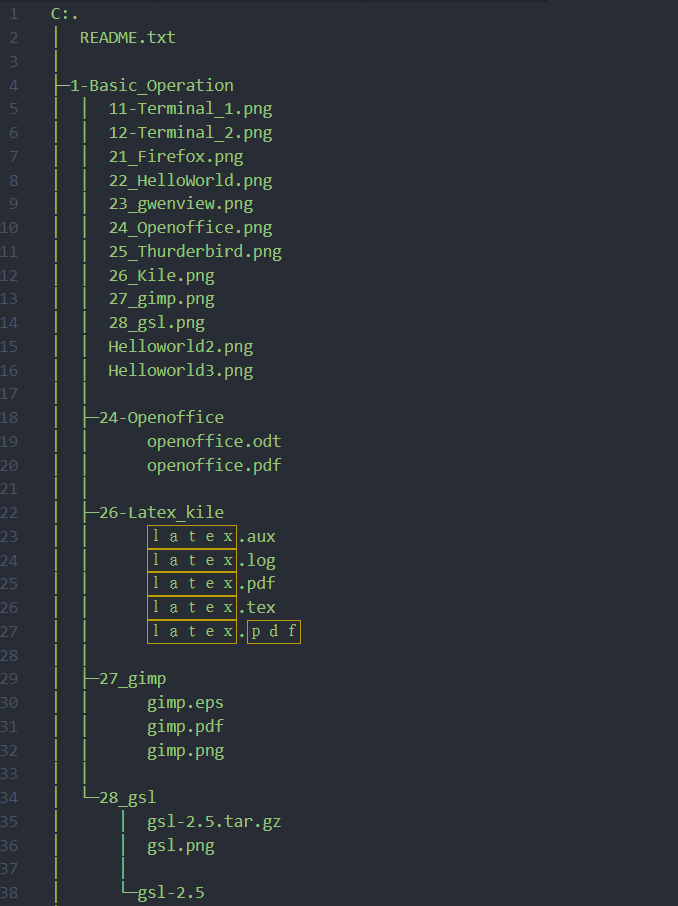
\includegraphics[width=0.4\textwidth]{attachments/fig.s1.1.png}
        }
        \subfloat[]{\label{fig:s1.2}
        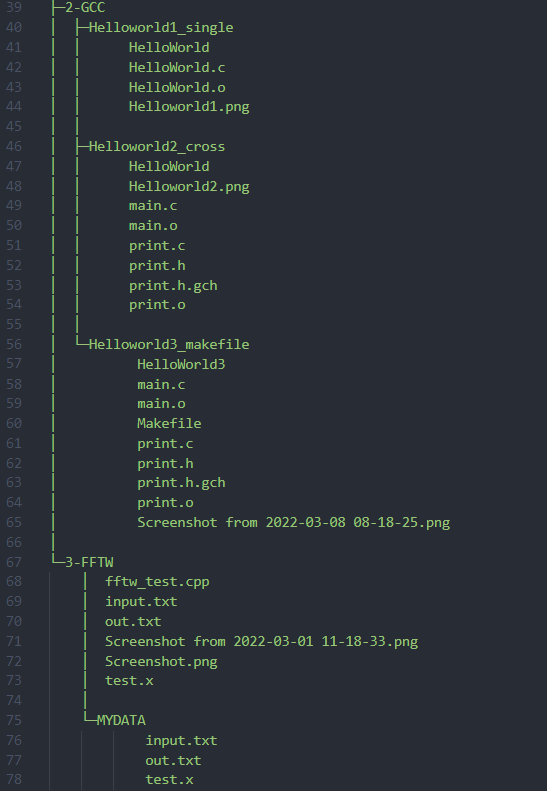
\includegraphics[width=0.4\textwidth]{attachments/fig.s1.2.png}
        }
        \caption{\textbf{Screenshots and output files in Exp.1}}
    \end{figure}

    Note: the data used in "3-FFTW/MYDATA" for the fftw computation are real-world data truncated from the electroencephalogram (EEG) signal
    of an epilepsy patient. Using $scipy.fftpack$ we can perform fast fourier transform in Python. The results is shown in Fig. \ref{fig:s1.3} and Fig. \ref{fig:s1.4}.
    \begin{figure}[htbp]
        \centering
        \subfloat[Original signal]{\label{fig:s1.3}
        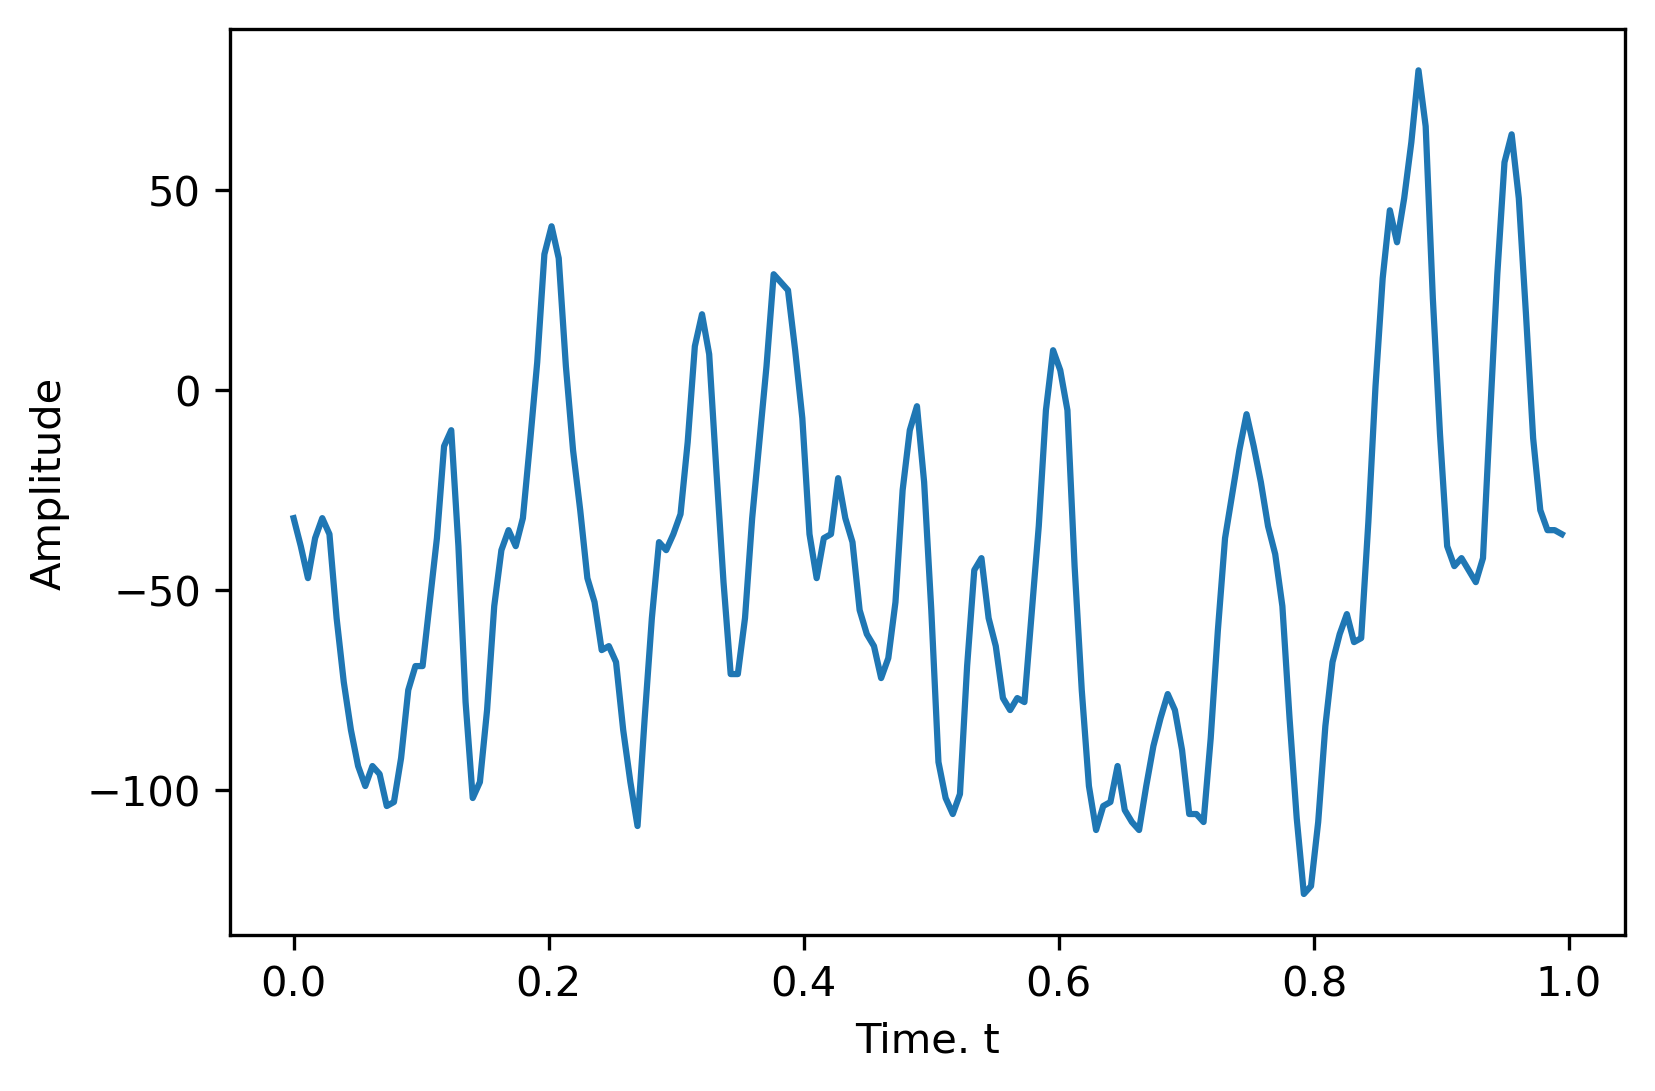
\includegraphics[width=0.4\textwidth]{attachments/fig.s1.3.png}
        }
        \subfloat[FFT output]{\label{fig:s1.4}
        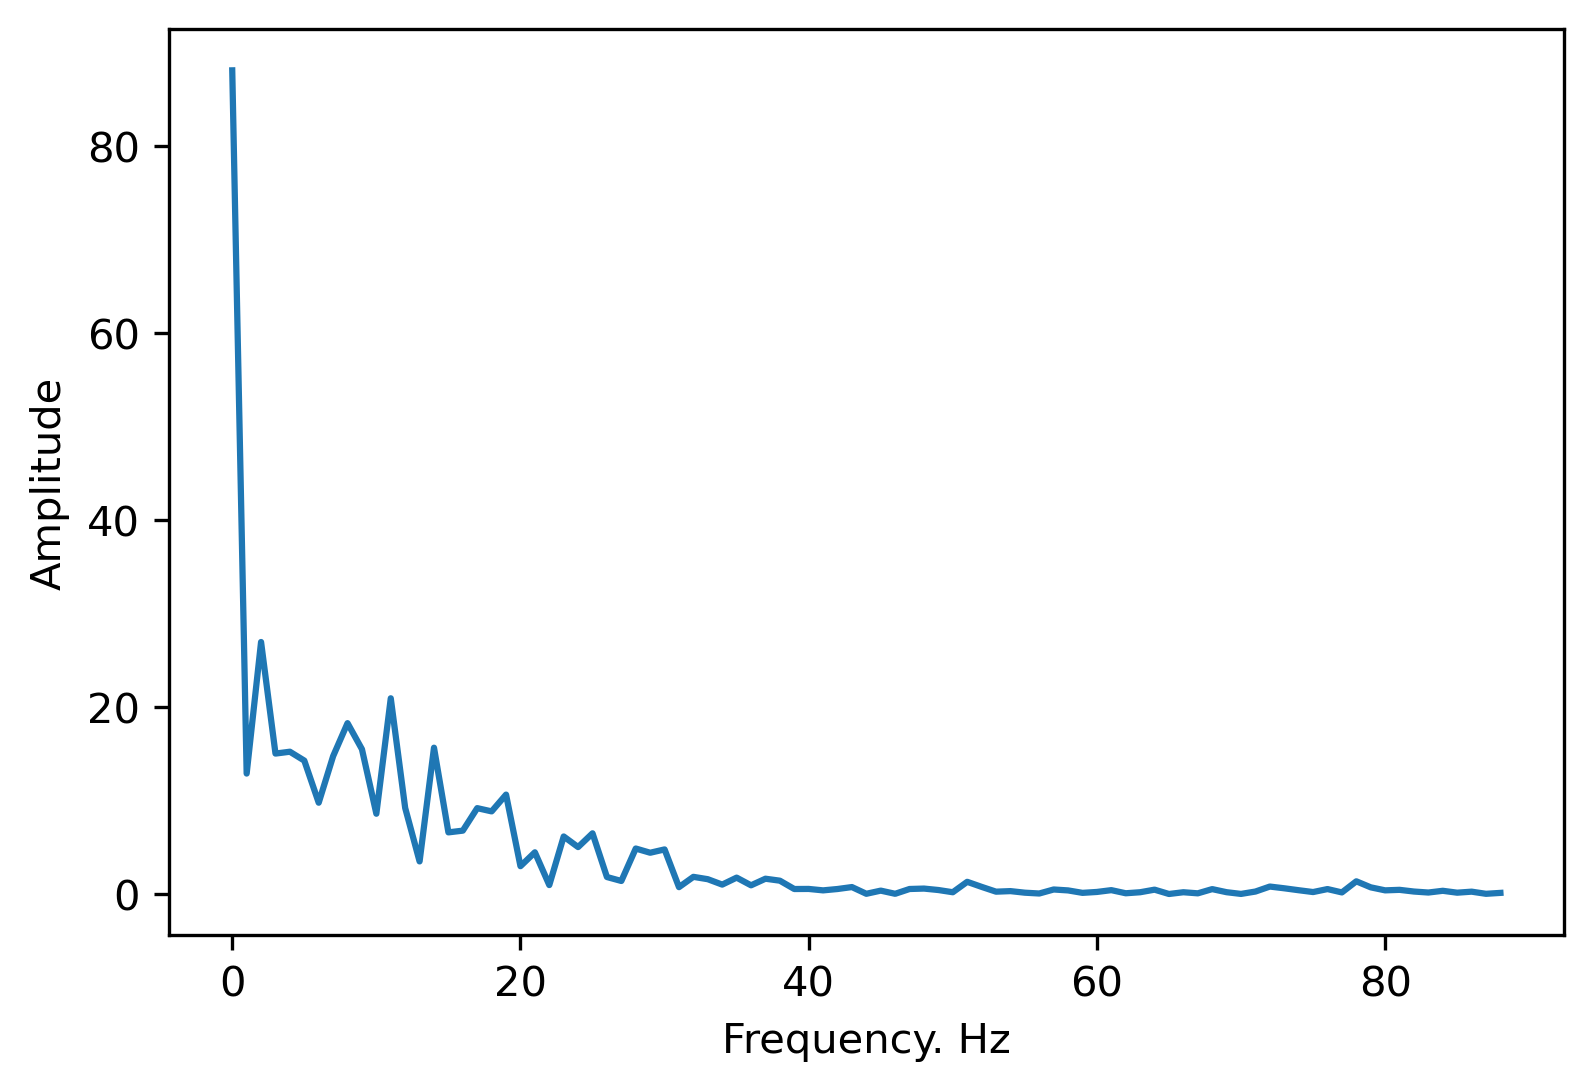
\includegraphics[width=0.4\textwidth]{attachments/fig.s1.4.png}
        }
        \caption{\textbf{Fast fourier transform of the real-world EEG data with $scipy.fftpack$}}
    \end{figure}

    \subsection{Question: Usage of the fftw library}
    The Fastest Fourier Transform in the West (fftw) library is a comprehensive collection 
    of fast C routines for computing the discrete Fourier transform (DFT) in one or more dimensions, 
    of both real and complex data, and of arbitrary input size.
    It provides functions for four modes of transformation: complex one-dimensional transforms, complex multi-dimensional transforms,
    real one-dimensional transforms, and real multi-dimensional transforms.

    The detailed usage can be found in \url{http://www.fftw.org/fftw2_doc/fftw_3.html}


\section{Exp.2 Python basic operation}
    \subsection{Main parameters}
    \begin{table}[htbp]
        \centering
            \begin{tabular}{cc}
                \toprule
                Item &parameters  \\
                \midrule
                Python &3.9.7 \\
                \bottomrule
            \end{tabular}
            \caption{\textbf{Parameters adopted in Exp. 2}}
            \label{tab:2.1}
    \end{table}	

    \subsection{Supplementary data and figure}
    All codes and results are illustrated in the Notebook "C10.2.ipynb", which together with all output files has been uploaded onto the server.
    
    Note: Beside using the basic graphics engine in python, I also used an advanced drawing package "$Seaborn$"(\url{https://seaborn.pydata.org/}) 
    to perform the statistics much elegentlier. Some results are illustrated in Fig. \ref{fig:s2.1} Fig. \ref{fig:s2.2} Fig. \ref{fig:s2.3.1} and Fig. \ref{fig:s2.3.2}.

    \begin{figure}[htbp]
        \centering
        \subfloat[ ]{\label{fig:s2.1}
        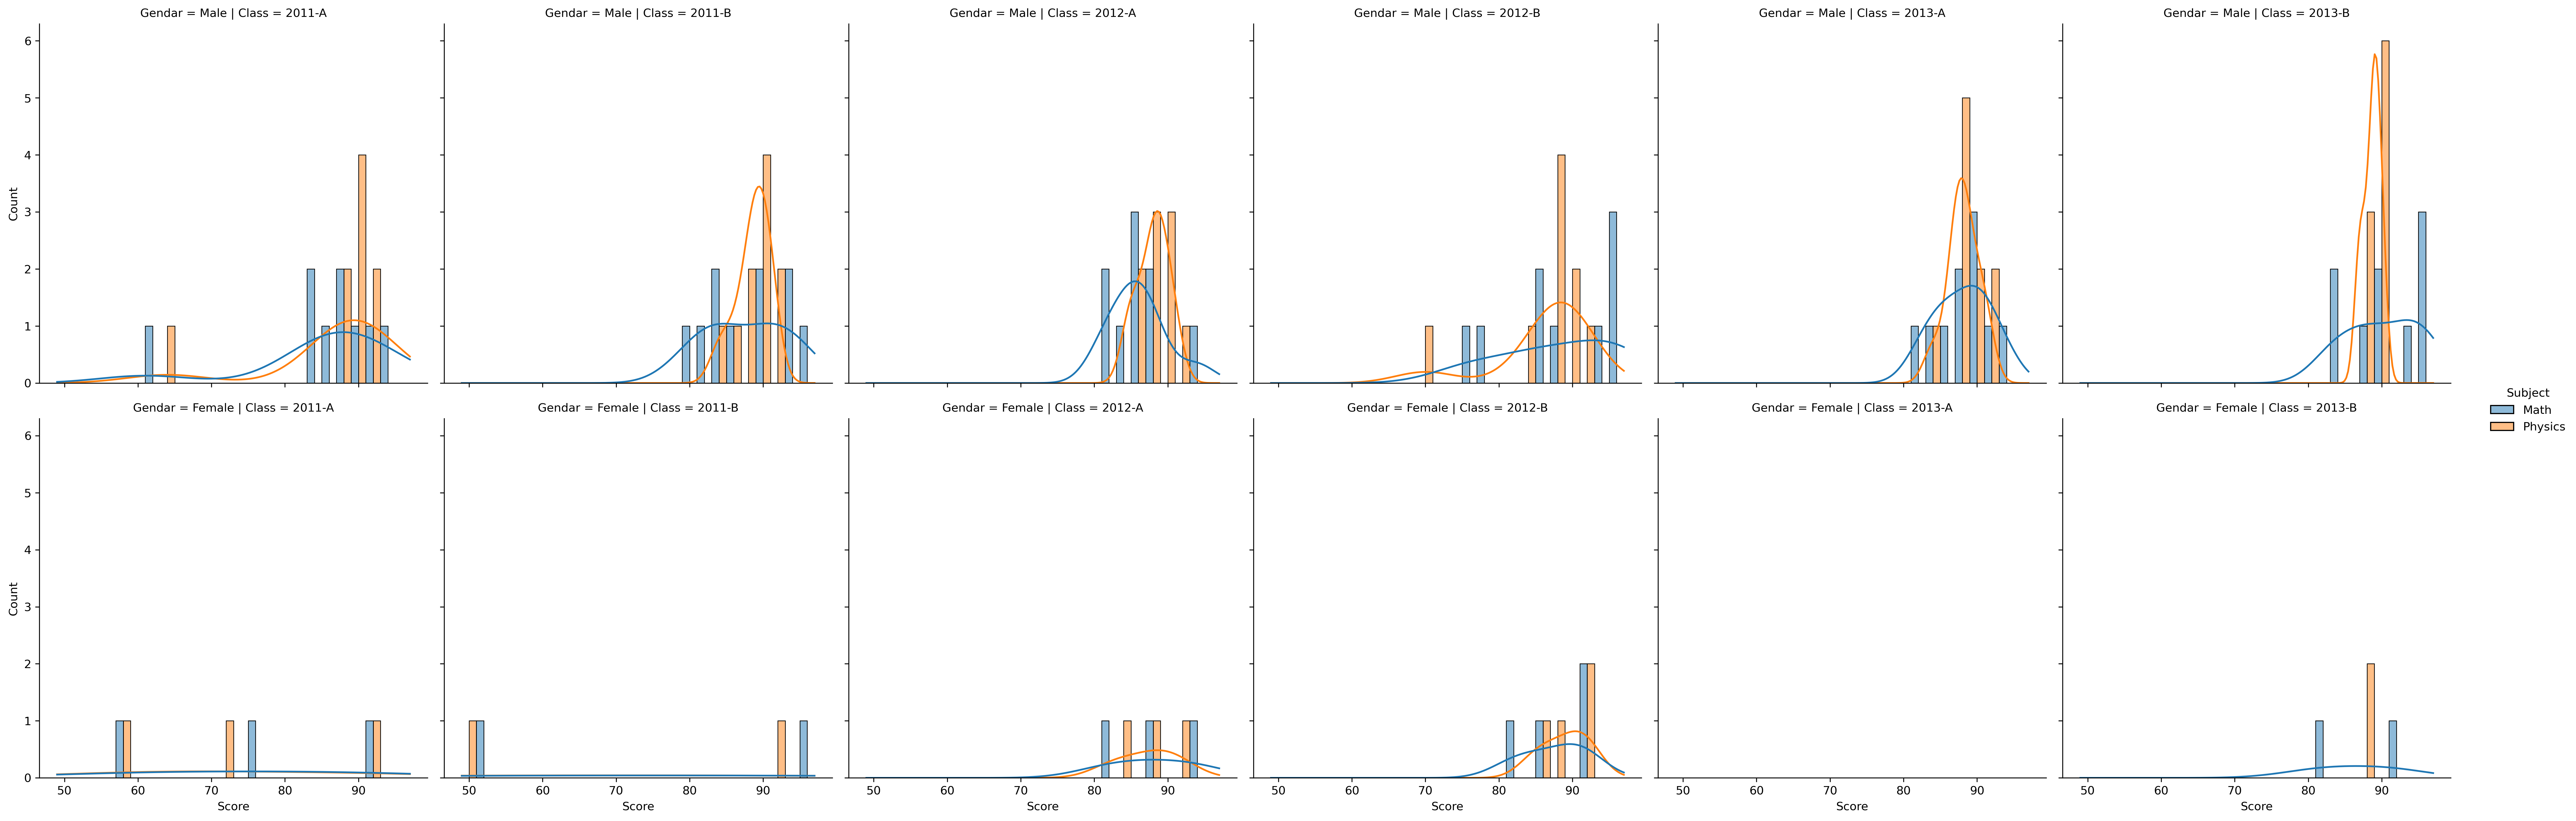
\includegraphics[width=0.4\textwidth]{attachments/fig.s2.1.png}
        }
        \subfloat[ ]{\label{fig:s2.2}
        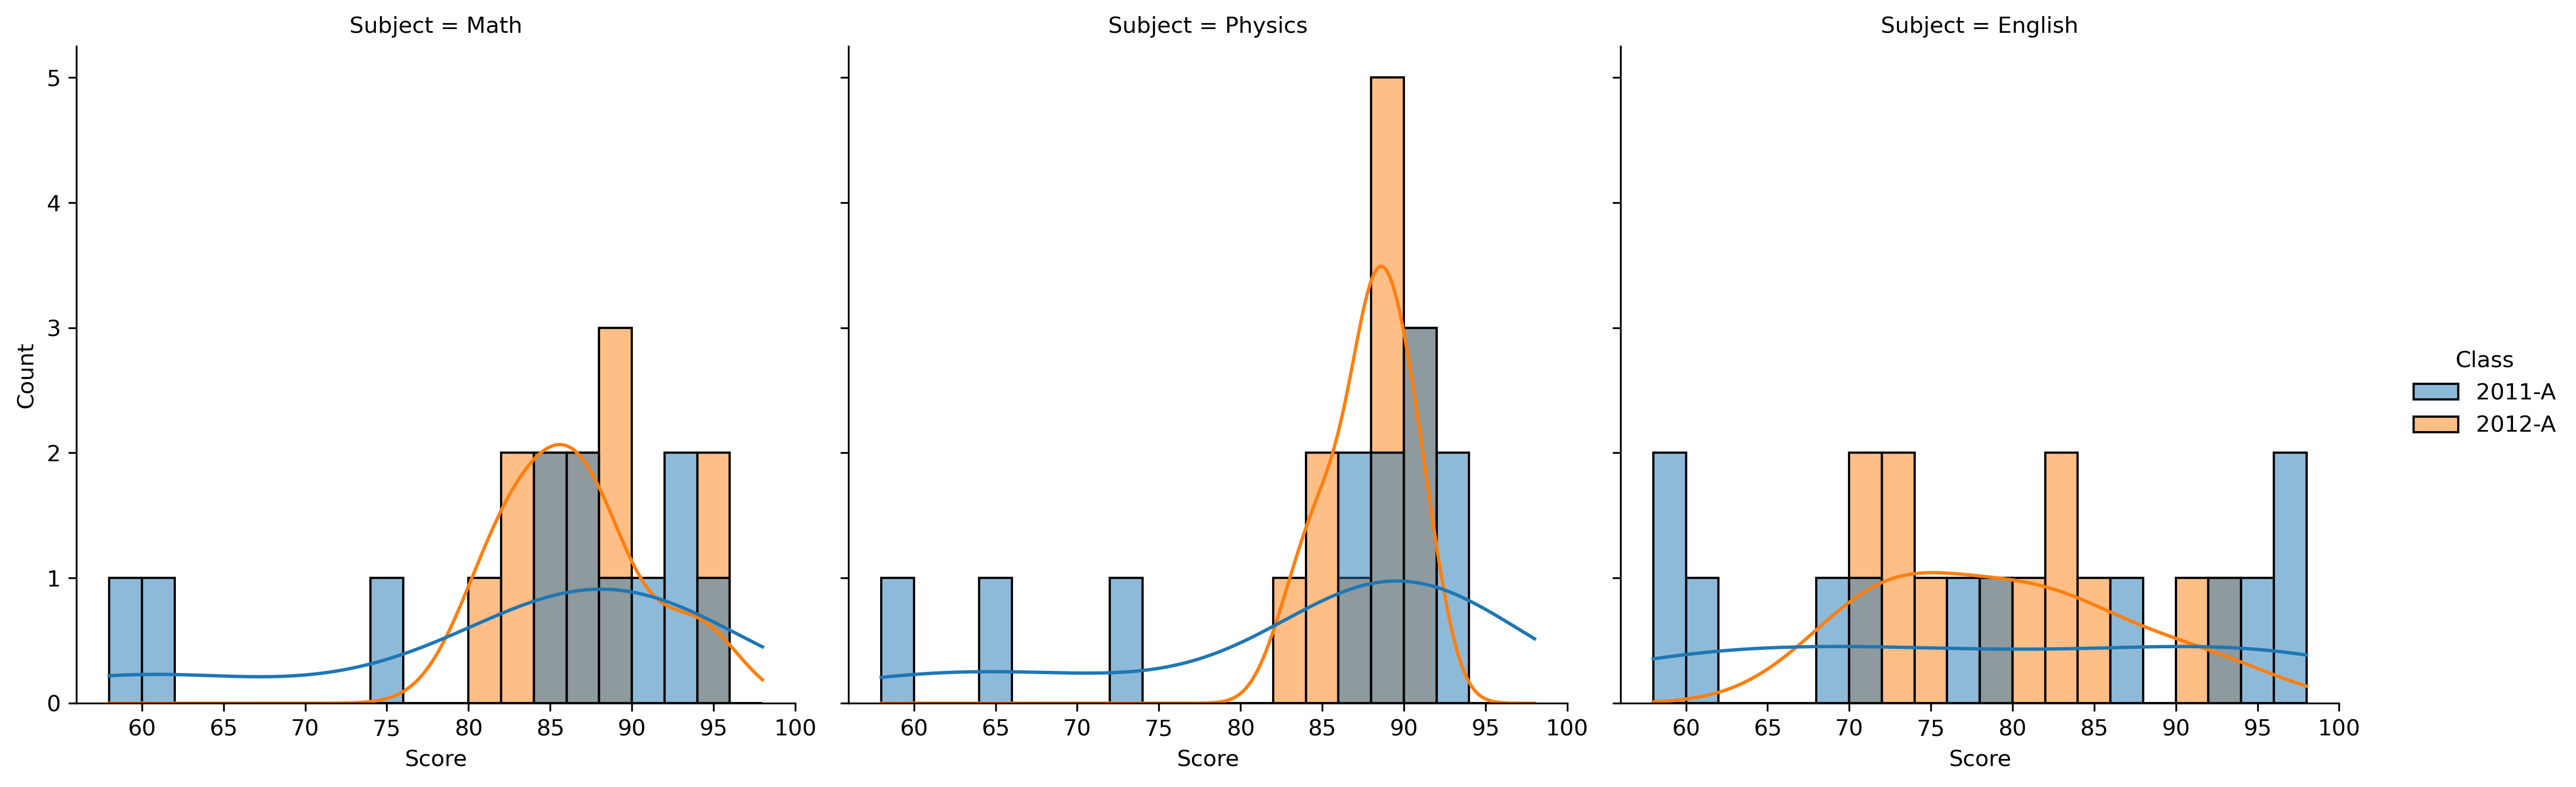
\includegraphics[width=0.4\textwidth]{attachments/fig.s2.2.png}
        }

        \subfloat[ ]{\label{fig:s2.3.1}
        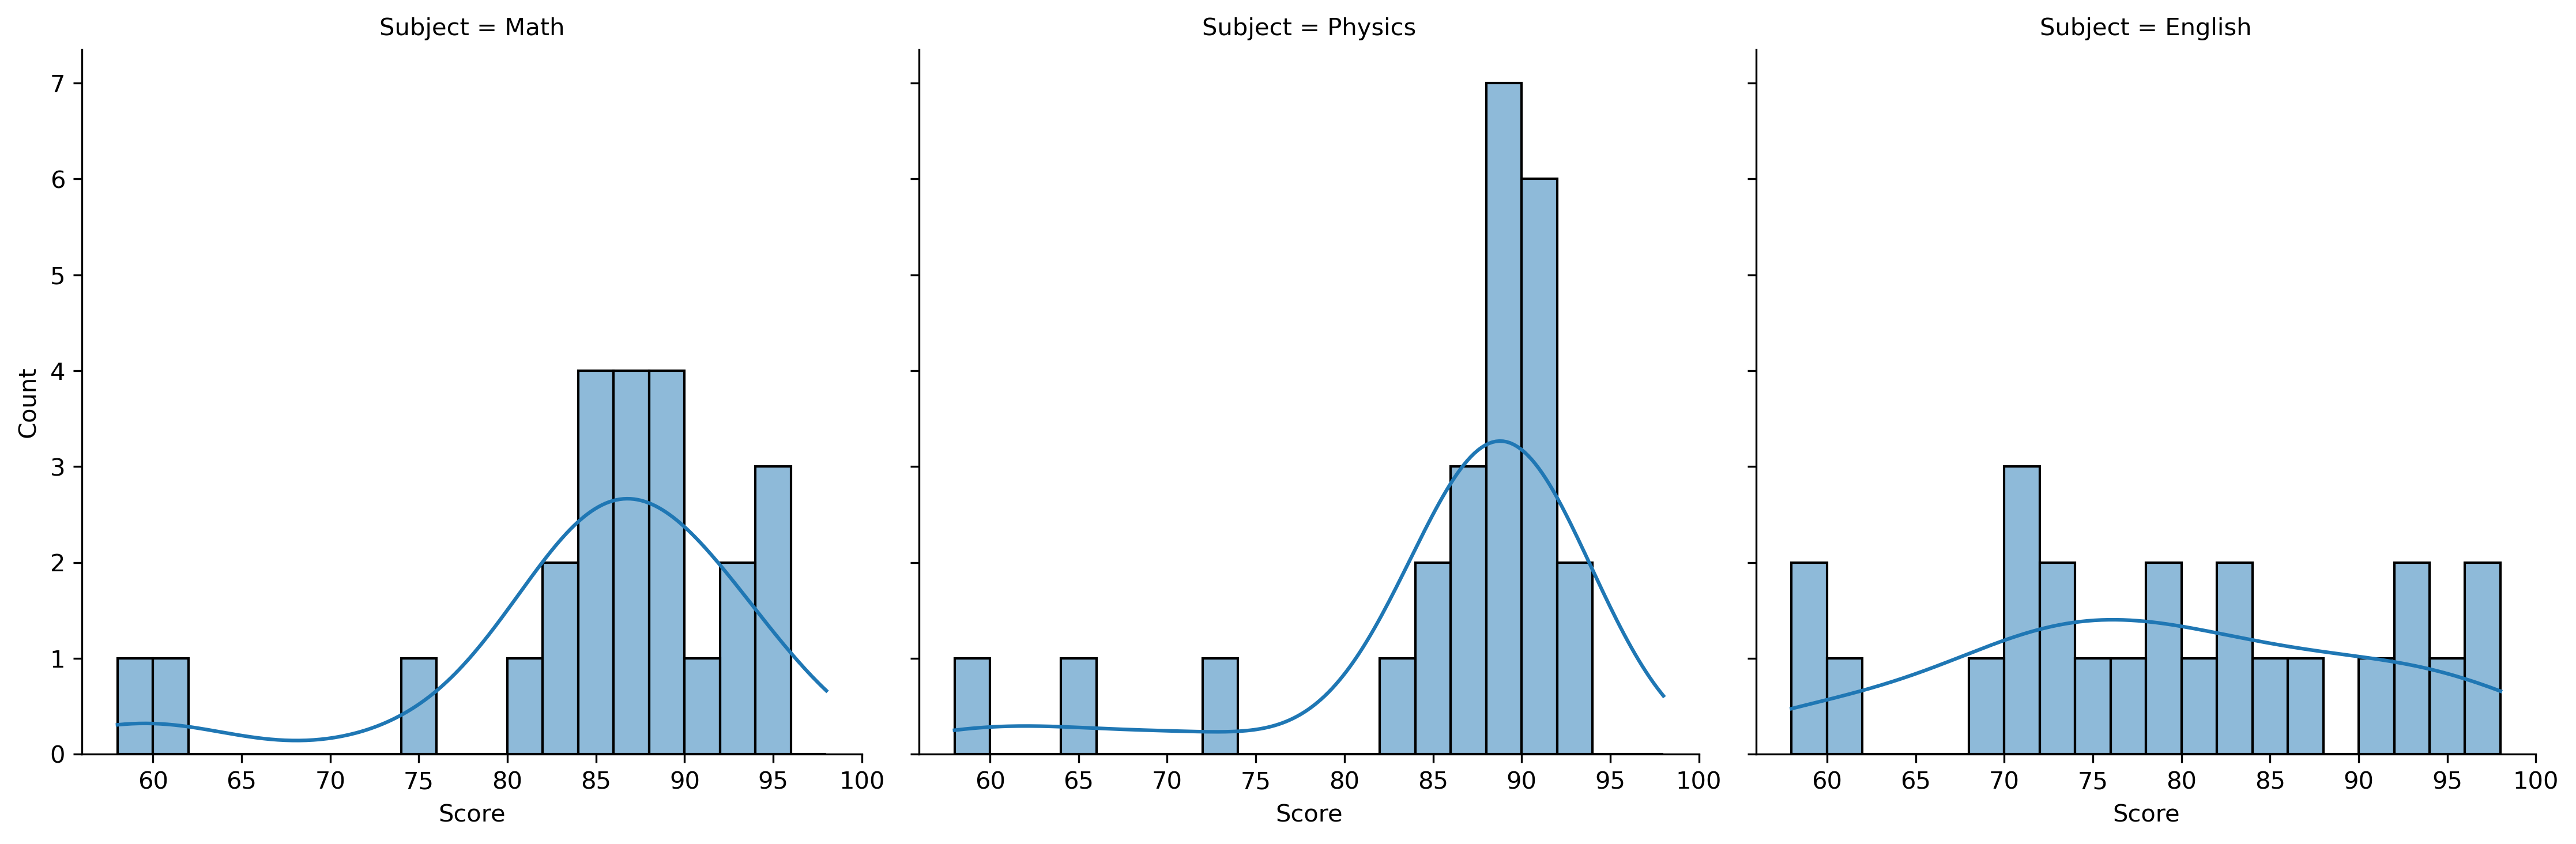
\includegraphics[width=0.4\textwidth]{attachments/fig.s2.3.1.png}
        }
        \subfloat[ ]{\label{fig:s2.3.2}
        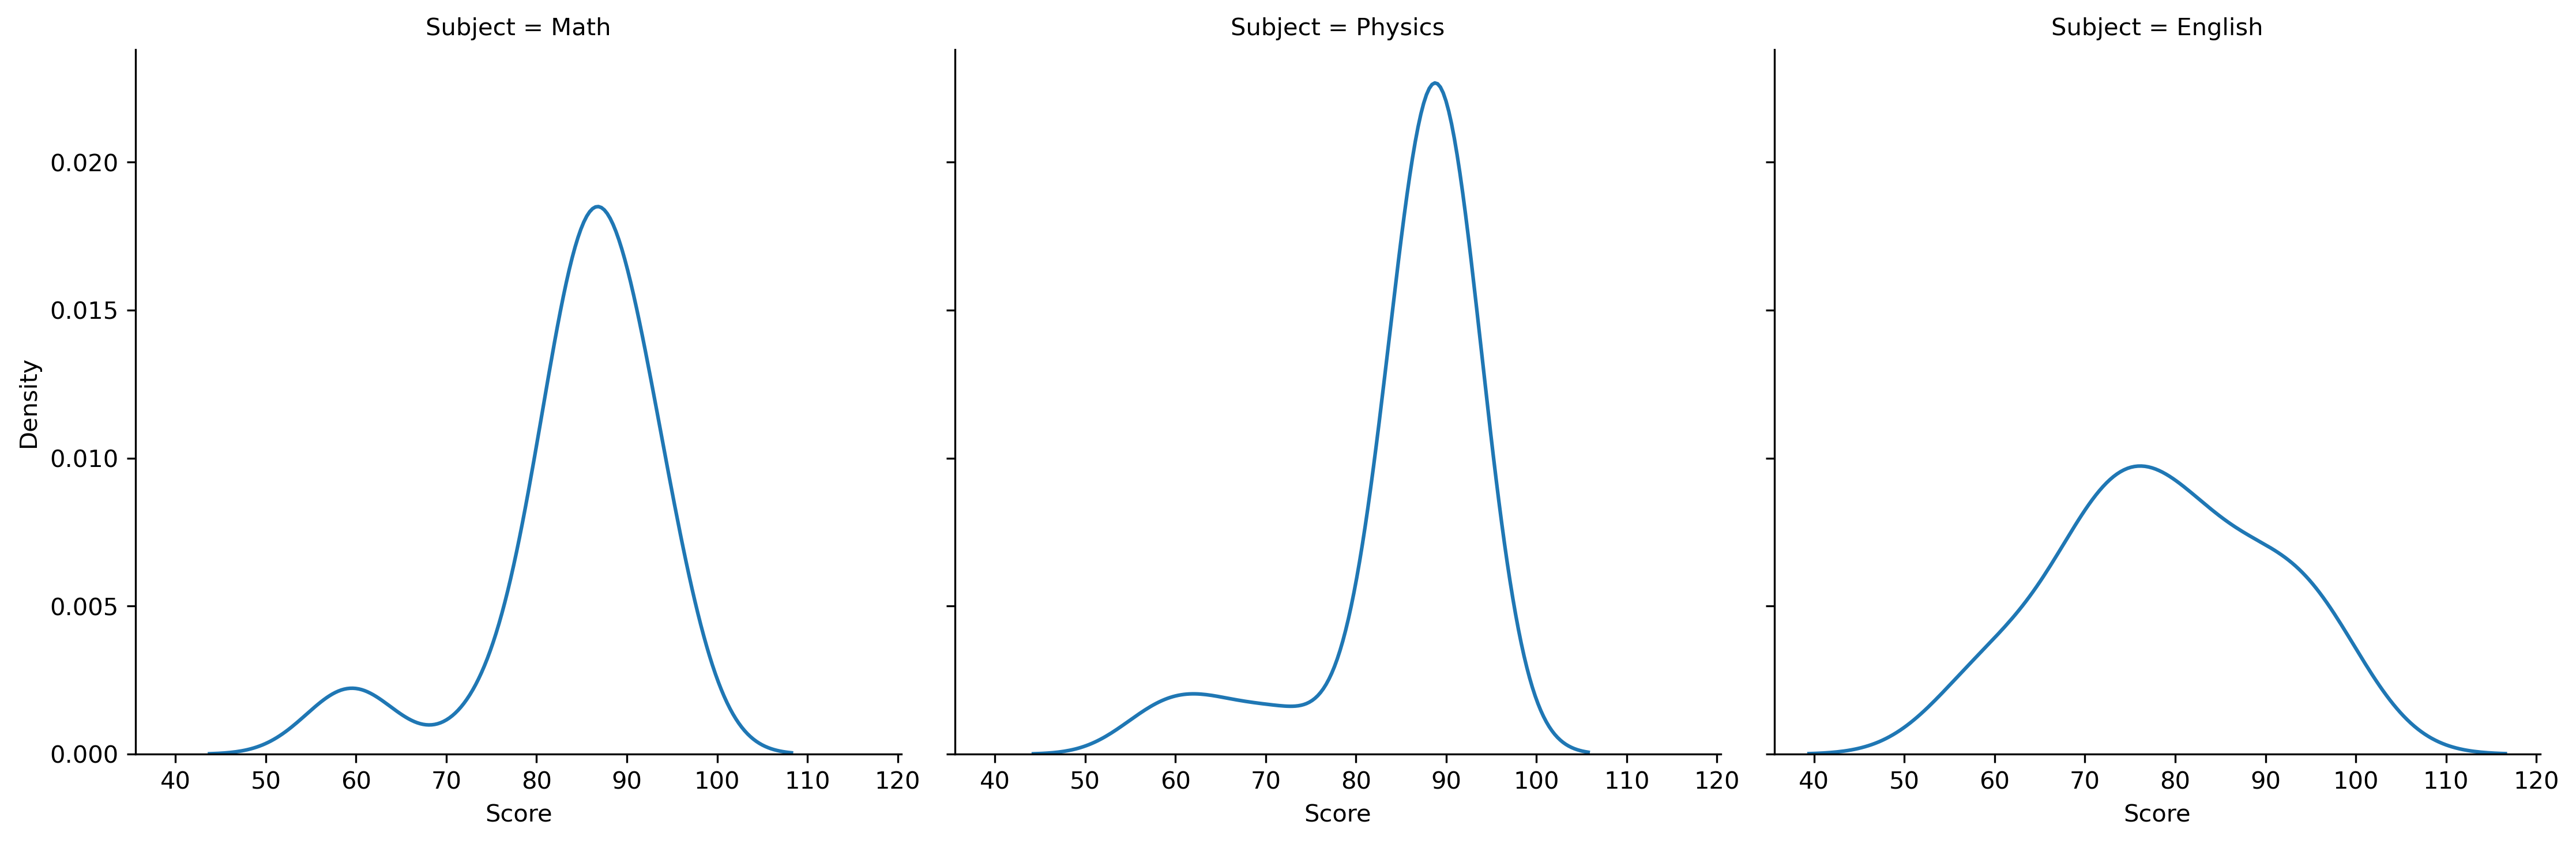
\includegraphics[width=0.4\textwidth]{attachments/fig.s2.3.2.png}
        }
        \caption{\textbf{Statistics performed with $Seaborn$}}
    \end{figure}

    \subsection{Question: Fast fourier transform of the Oscillation attenuation signal}
    The method of performing fast fourier transform on a signal has been illustrated in the Notebook.
    To be brief, I use $fftfreq$ to calculate the frequency, and $fft$ to calculate the amplitude of every frequency.
    These functions are implanted in $scipy.fftpack$. The results are shown in Fig. \ref{fig:s2.4.1} and Fig. \ref{fig:s2.4.2}
    \begin{figure}[htbp]
        \centering
        \subfloat[The original signal]{\label{fig:s2.4.1}
        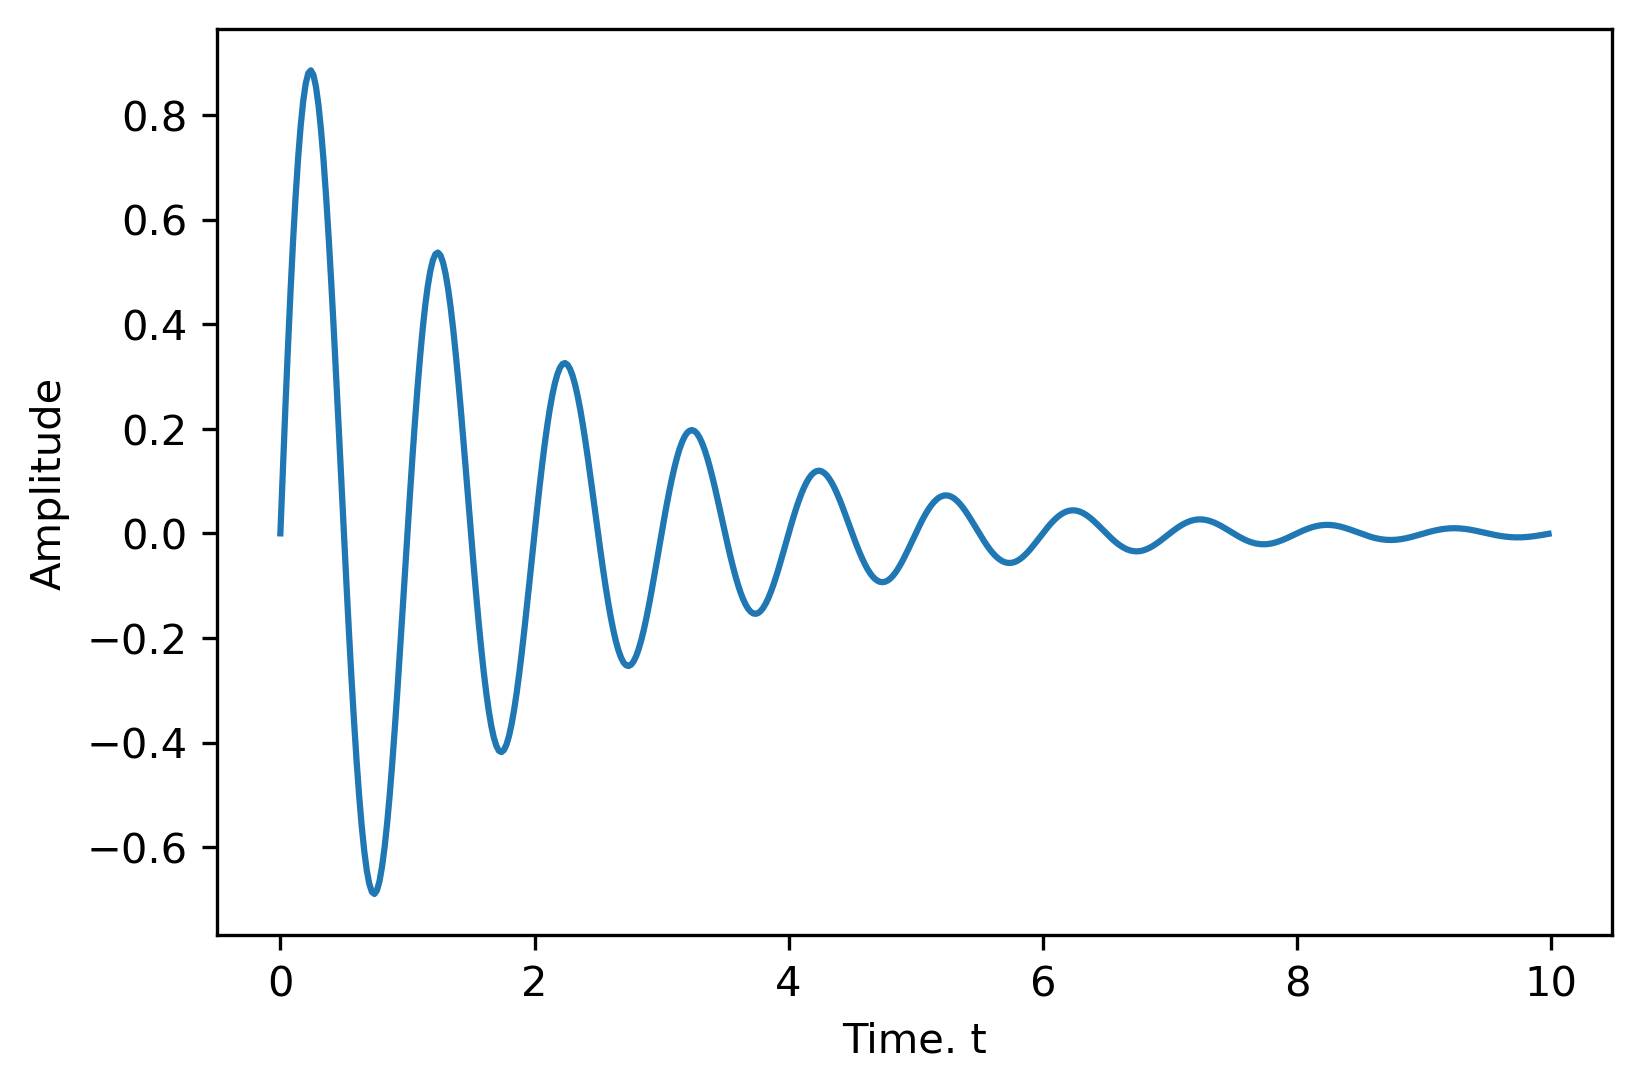
\includegraphics[width=0.4\textwidth]{attachments/fig.s2.4.1.png}
        }
        \subfloat[FFT result]{\label{fig:s2.4.2}
        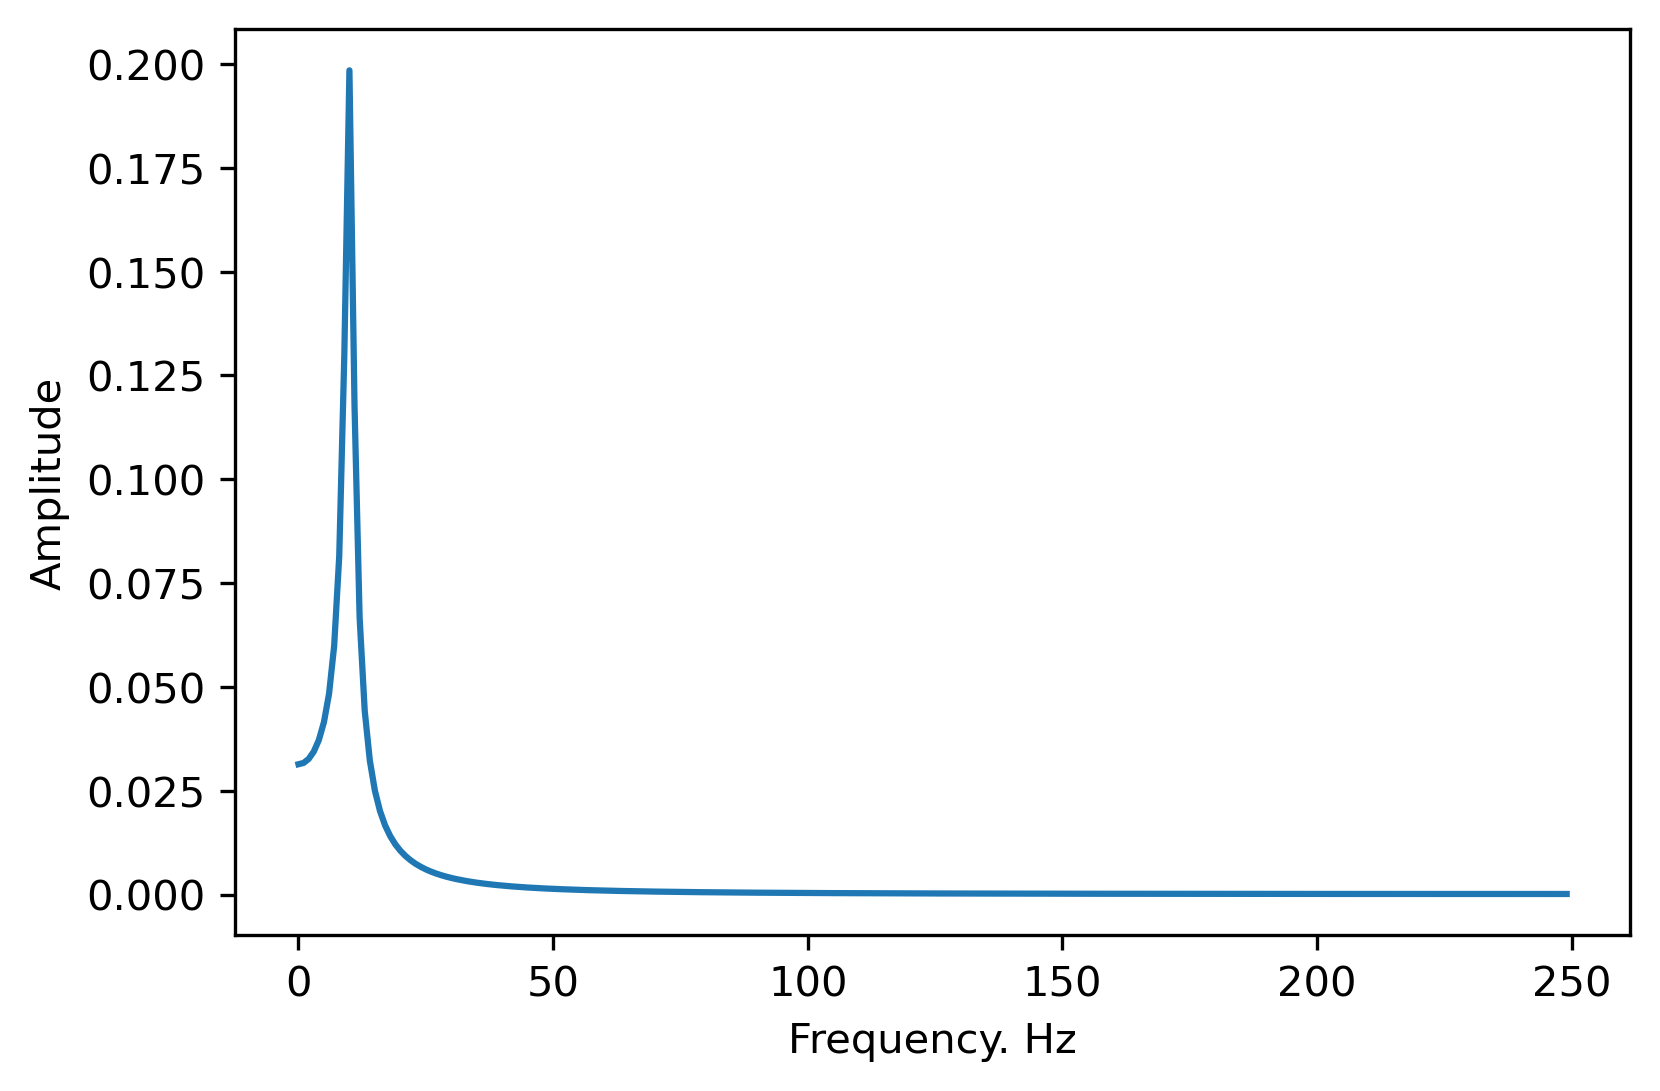
\includegraphics[width=0.4\textwidth]{attachments/fig.s2.4.2.png}
        }
        \caption{\textbf{Fast fourier transform of the Oscillation attenuation signal}}
    \end{figure}


\section{Exp.3 Maximum likelihood estimate}
    \subsection{Main parameters}
    \begin{table}[htbp]
        \centering
            \begin{tabular}{cc}
                \toprule
                Item &parameters  \\
                \midrule
                Python &3.9.7 \\
                numpy  &1.20.3 \\
                pandas  &1.3.4 \\
                scipy  &1.7.1 \\
                matplotlib  &3.4.3 \\
                seaborn  &.11.2 \\           
                \bottomrule
            \end{tabular}
            \caption{\textbf{Parameters adopted in Exp. 3}}
            \label{tab:3.1}
    \end{table}	

    \subsection{Supplementary data and figure}
        \subsubsection{Confidence intervals of different data}
        \begin{table}[htbp]
                \centering
                    \begin{tabular}{ccccc}
                        \toprule
                        Item &Setting & Estimate & + & - \\
                        \midrule
                        Data\_1-A events &100   & 92.84 & +12.63 & -11.89 \\
                        Data\_1-B events &200   & 207.16 & +16.65 & -15.88 \\
                        Data\_2\_1-A events &150    & 139.90 & +14.98 & -14.26 \\
                        Data\_2\_1-B events &200    & 210.10 & +17.25 & -16.45 \\
                        Data\_2\_2-A events &200    & 205.62 & +16.79 & -16.11 \\
                        Data\_2\_2-B events &200    & 194.38 & +16.51 & -15.70 \\
                        Data\_2\_3-A events &250    & 249.20 & +18.62 & -17.92 \\
                        Data\_2\_3-B events &200    & 200.80 & +17.31 & -16.48 \\
                        Data\_2\_4-A events &300    & 310.35 & +20.18 & -19.49 \\
                        Data\_2\_4-B events &200    & 189.65 & +16.93 & -16.09 \\
                        Data\_3\_1-A events &50    & 43.88 & +8.90 & -8.17 \\
                        Data\_3\_1-B events &100    & 106.12 & +12.01 & -11.23 \\
                        Data\_3\_2-A events &75    & 78.33 & +11.44 & -10.71 \\
                        Data\_3\_2-B events &150    & 146.67 & +14.21 & -13.43 \\
                        Data\_3\_3-A events &125    & 124.16 & +14.62 & -13.88 \\
                        Data\_3\_3-B events &250    & 250.84 & +18.55 & -17.77 \\
                        Data\_3\_4-A events &150    & 161.35 & +16.35 & -15.62 \\
                        Data\_3\_4-B events &300    & 288.65 & +19.96 & -19.17 \\
                        \bottomrule
                    \end{tabular}
                    \caption{\textbf{Confidence intervals of different data}}
                    \label{tab:3.2}
        \end{table}	
        
        Note: All these data and the corresponding output have been uploaded to the server. 
        The workflow was designed to allow reproduce the outputs easily. See the Notebook "C10.3.ipynb" for details.

        \subsubsection{The regression parameters of the confidence intervals}

        \paragraph{Change the proportion.} Class A: $y = 0.069x+18.853; r=0.994$; Class B does not show a linear correlation.
        \paragraph{Change the total number.} Class A: $y = 0.127x+12.075; r=0.994$; Class B: $y = 0.086x+14.535; r=0.998$

    



\section{Data and code availability}
Data and code are available at \url{https://github.com/Jeg-Vet/SYSU-PHY-EXP/tree/main/}

\end{document}